\section{Zhodnotenie}
\indent \indent V tejto sekcií predstavíme výsledok našej práce. Webovú aplikáciu sme nasadili na verejný server, aby sme ju mohli odovzdať na testovanie reálnym používateľom. Týmto spôsobom získame objektívnu odozvu a hodnotenie našej aplikácie.
\subsection{Výsledok práce}

\indent \indent Vytvorili sme webovú aplikáciu pomocou knižnice \textit{Node.js}. Naštudovali sme trasovací engine \textit{Valhalla} a spôsoby jeho použitia. Funkcie, ktoré \textit{Valhalla} poskytuje sa nám podarilo integrovať do našej webovej aplikácie \textit{Routiak}. 

\indent Routiak je webová aplikácia, pomocou ktorej si môže používateľ vizualizovať vlastné trasy na mape prehľadne. To znamená, že aj pri veľkom počte trás (10 a viac) prechádzajúcich tým istým miestom, môže používateľ nastaviť zobrazenie tak, aby bolo prehľadné a na mape nevznikali tzv. "špagety"(obr.\ref{fig:spagety}). Vďaka správnemu nastaveniu zobrazenia je možné vidieť trasy a cestnú sieť prehľadne. Používateľ sa môže v aplikácii registrovať a prihlásiť a teda je možné nahrané trasy zobraziť neskôr bez nutnosti znova trasy do aplikácie nahrať. Trasy sa do aplikácie nahrávajú v ZIP súbore, čo umožňuje nahrať viac trás súčasne. Tieto trasy je možné zobraziť na mape jednotlivo, alebo všetky naraz obsiahnuté v ZIP súbore. Aplikácia ponúka map-match funkcionalitu, čo znamená, že trasy budú pripnuté na cestnú sieť a tým sa zlepší viditeľnosť mapy a trás na mape, obrázok \ref{fig:niespagety}. 
\newline Výhody:
\begin{itemize}
  \item map-match, pripnutie trás na cestnú sieť pre zlepšenie viditeľnosti
  \item možnosť nahrať viac trás naraz
  \item zobrazenie vlastných trás po nahratí bez nutnosti nahrávať trasy pri každom zobrazení
  \item možnosť nahrať trasy vo viacerých formátoch (CSV,GEOJSON,GPX)
  \item neobmedzený počet zobrazení mapy s neobmedzeným počtom nahraných súborov (počet nahraných súborov je obmedzený veľkosťou vyhradeného miesta na serveri)
  \item do jednej požiadavky na map-match môže ísť až 20 tisíc súradníc
  \item informácia pre používateľa v prípade, že niektorá z trás nemala požadovaný formát 
\end{itemize}
Nevýhody:
\begin{itemize}
  \item trasa môže obsahovať maximálne 20 tisíc bodov
  \item nie je možné pripnúť trasu zaznamenanú rôznymi typmi dopravy (auto + pešia chôdza)
  \item priebeh \textit{map-match} ZIP súboru nie je zobrazený, iba informácia po dokončení
  \item pri nahratí jednej trasy je nutné vložiť trasu do ZIP súboru so špeciálne určenou štruktúrou
\end{itemize}
\begin{figure}[H]
  \centering
  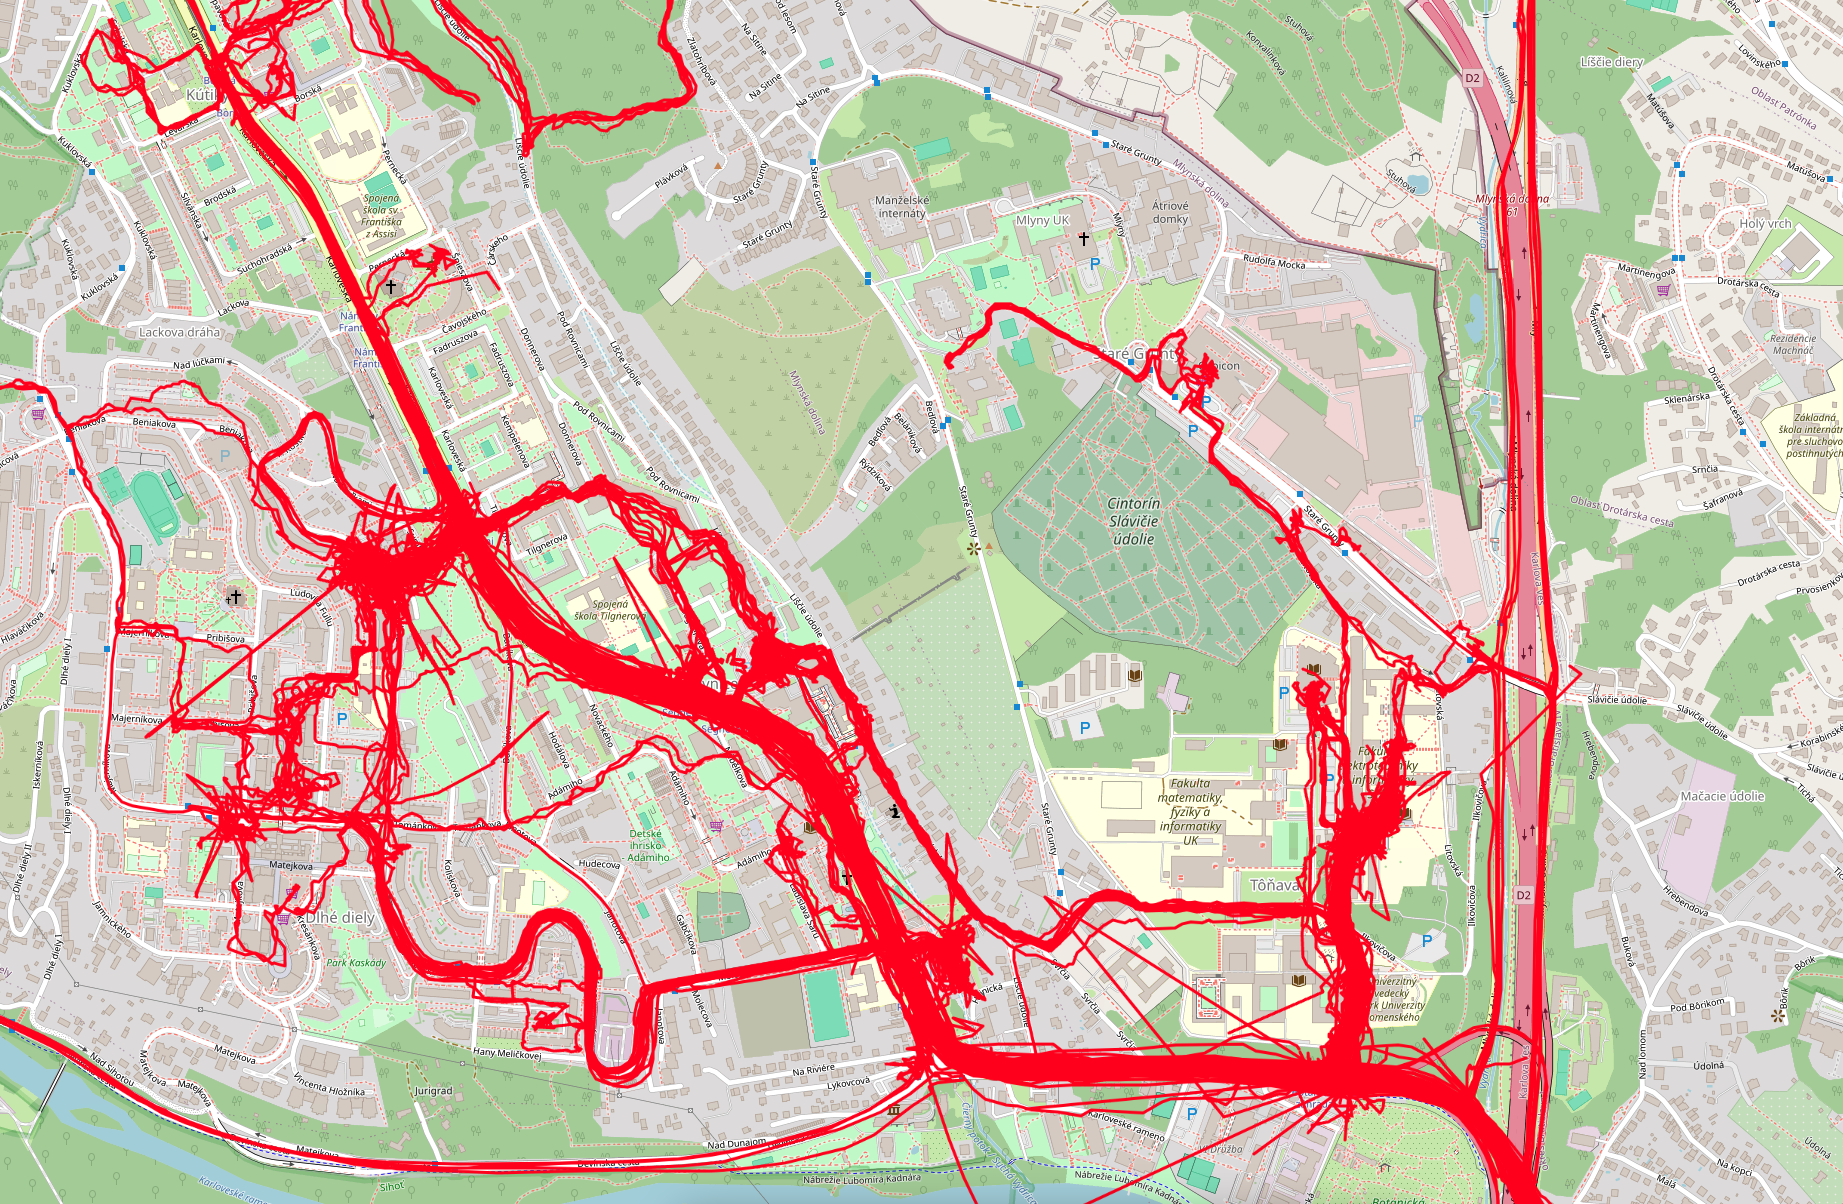
\includegraphics[width=0.7\textwidth]{img/map-match rozdiel/pred map-match.png}
  \caption{Zobrazenie väčšieho množstva trás na rovnakom mieste}
  \label{fig:spagety}
\end{figure}
\begin{figure}[H]
  \centering
  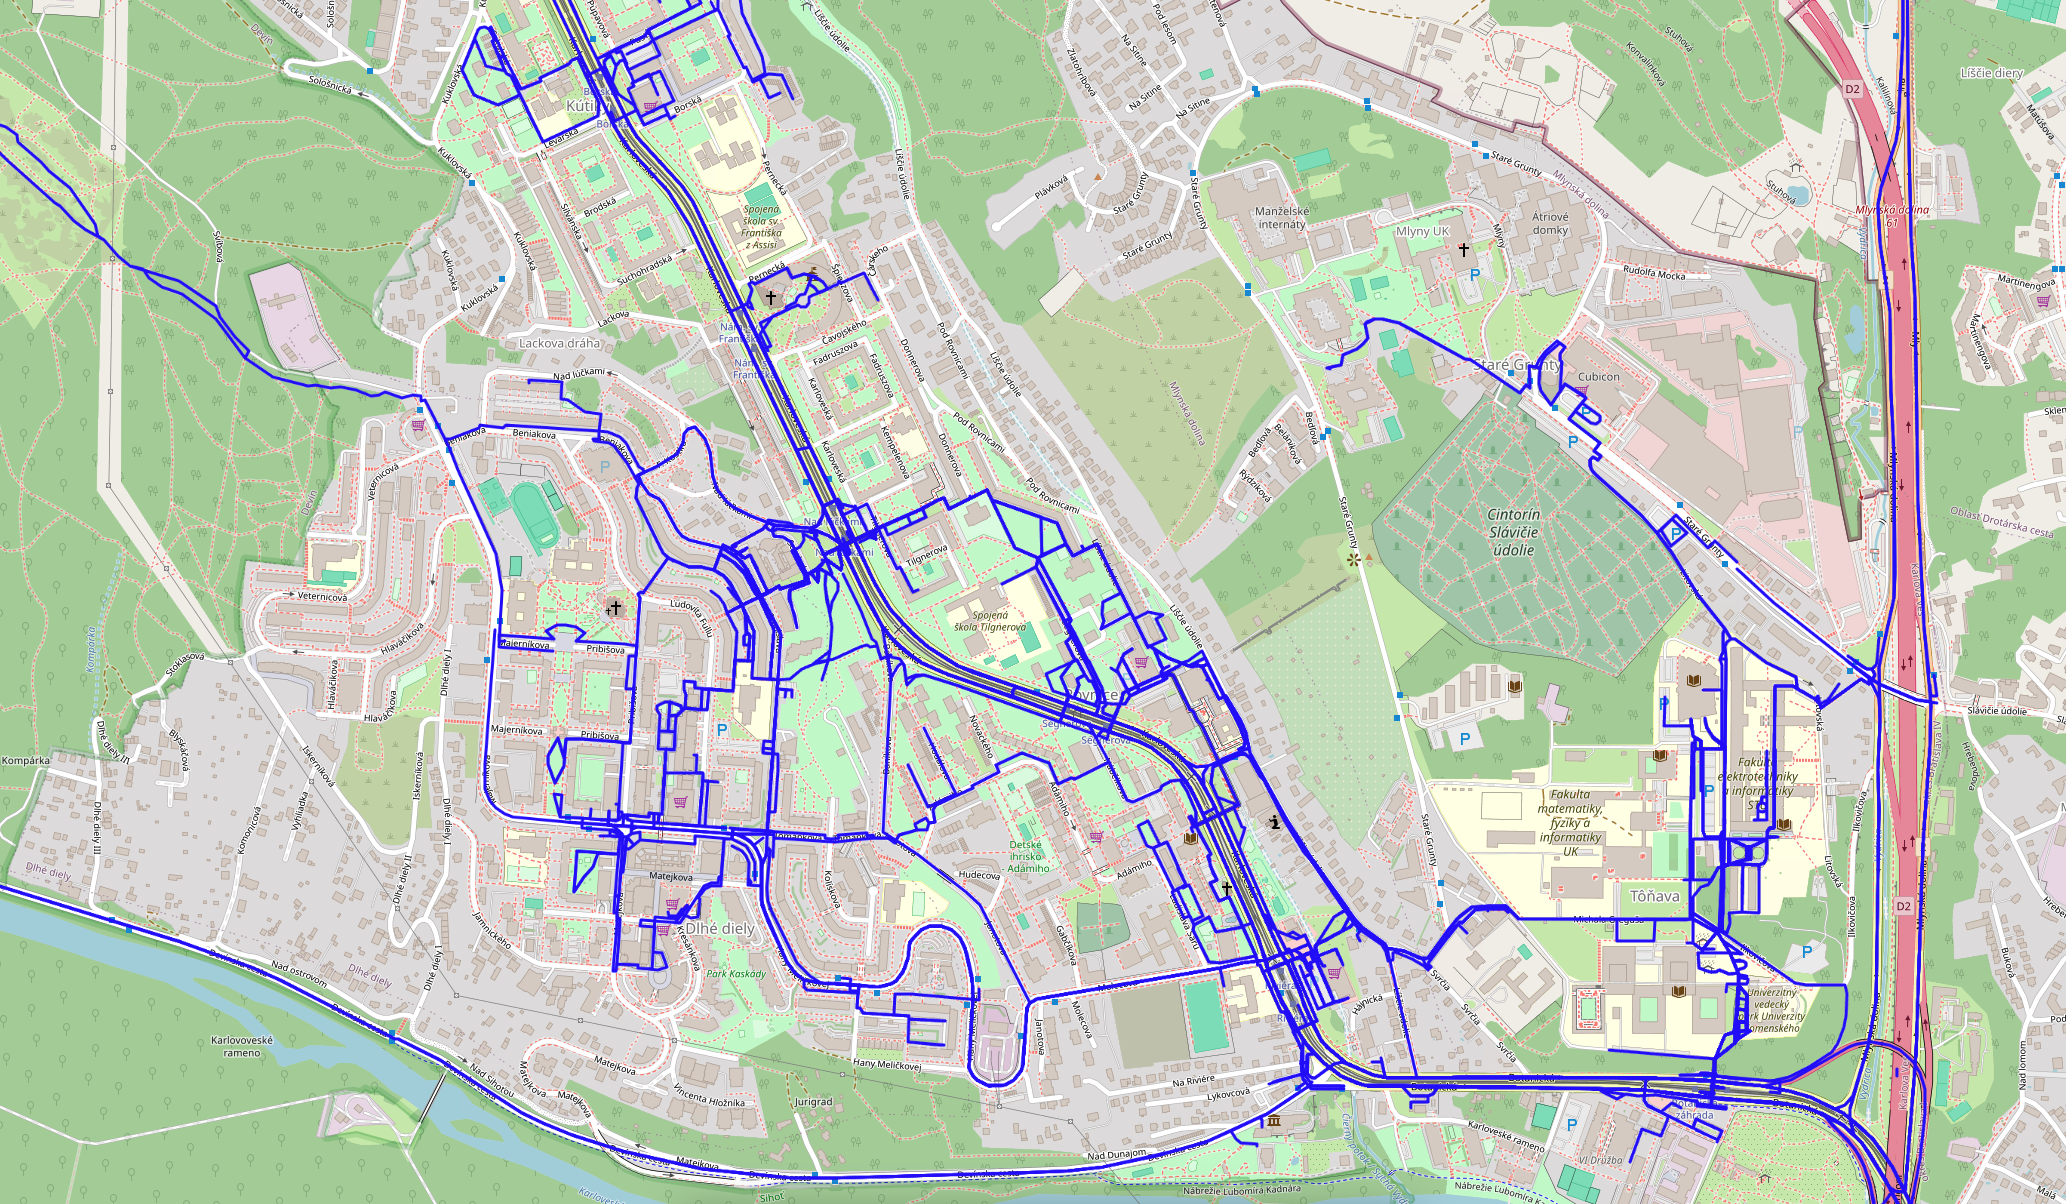
\includegraphics[width=0.7\textwidth]{img/map-match rozdiel/po map-match.png}
  \caption{Zobrazenie väčšieho množstva trás upravených map-matchom na rovnakom mieste}
  \label{fig:niespagety}
\end{figure}

\pagebreak
\subsection{Hodnotenie práce reálnymi používateľmi}
Sem pojde dotaznicek TODO

